%\documentclass{article}
\documentclass{report}
%\usepackage[utf8]{vietnam}
\usepackage[utf8]{inputenc}
\usepackage{anyfontsize,fontsize}
\changefontsize[13pt]{13pt}	
\usepackage{commath}
\usepackage{parskip,setspace}
\usepackage{xcolor}
\usepackage{amssymb}
\usepackage[d]{esvect}
\usepackage{slashed,cancel}
\usepackage{indentfirst,titlesec}
\usepackage{pdfpages}
\usepackage{graphicx,subcaption,floatrow}
\usepackage{nccmath}
\usepackage{mathtools}
\usepackage{amsfonts}
\usepackage{amsmath,systeme}
\usepackage[thinc]{esdiff}
\usepackage{hyperref,tikz}
\usepackage{bm,physics,nicematrix}
\usepackage[super,comma]{natbib}
%footnote
\usepackage{fancyhdr}
\usepackage{array,tocbibind}

\pagestyle{empty}


\usepackage{geometry}
\geometry{
	a4paper,
	total={170mm,257mm},
	left=20mm,
	top=20mm,
}



\newcommand{\image}[1]{
	\begin{center}
		\includegraphics[width=0.5\textwidth]{pic/#1}
	\end{center}
}




\renewcommand{\l}{\ell}
\newcommand{\dps}{\displaystyle}

\newcommand{\f}[2]{\dfrac{#1}{#2}}
\newcommand{\at}[2]{\bigg\rvert_{#1}^{#2} }


\renewcommand{\baselinestretch}{2.0}



\hypersetup{
	colorlinks=true,
	linkcolor=black,
	filecolor=magenta,      
	urlcolor=cyan,
	pdftitle={UT},
	citecolor=black,
	pdfpagemode=FullScreen,
}

\urlstyle{same}

\titleformat{\chapter}[display]
{\centering\large\bfseries} 
{\textbf{\MakeUppercase{\chaptername}} \ \thechapter\vspace{15pt}}{20pt}
{\large} 

\newcommand{\thesistitlee}{Three-band tight biding model for TMD monolayers in the presence of a magnetic field}
\newcommand{\address}{NATIONAL UNIVERSITY OF HO CHI MINH CITY UNIVERSITY OF SCIENCE}
\newcommand{\department}{FACULTY OF PHYSICS - ENGINEERING PHYSICS}
\newcommand{\thesisauthor}{Tran Khoi Nguyen}
\newcommand{\thesisadvisor}{Your Advisor's Name}
\newcommand{\graddate}{Ho Chi Minh City, 2025}
\newcommand{\thesisdedication}{To all the Ph.D. pursuing brave souls}


\begin{document}
\setlength{\parindent}{20pt}
\begin{center}
	{\bfseries

		{\large {\bf \address}}\\
		\vspace{2.5cm}

		{\large {\bf UNDERGRADUATE THESIS}}\\
		\vspace{3.0cm}


		{\largerrr\thesistitlee}
		\vspace{1in}

		{\large\graddate}
	}

\end{center}
\noindent
\makebox[\textwidth]{\hfill\makebox[3in]{\hrulefill}}\\
\begin{center}
	\makebox[\textwidth]{\hfill\makebox[3in]{\hfill \textbf{Sutdent: Tran Khoi Nguyen}\hfill}}
	\makebox[\textwidth]{\hfill\makebox[3in]{\hfill \textbf{Supervisor: Dr. Huynh Thanh Duc}\hfill}}
\end{center}
\begin{tikzpicture}[remember picture, overlay]
	\draw[line width=2pt]
	([xshift=1.5cm, yshift=1.5cm] current page.south west)
	rectangle
	([xshift=-1.5cm, yshift=-1.5cm] current page.north east);
\end{tikzpicture}
\newpage
\pagestyle{fancy}
\renewcommand{\headrulewidth}{0pt}
\fancyhf{}
\fancyfoot[C]{\hspace{0cm} \thepage}
\setcounter{page}{1}
\renewcommand{\contentsname}{TABLE OF CONTENTS}
\tableofcontents
\renewcommand{\listfigurename}{LIST OF FIGURES}
\listoffigures
\chapter{\textbf{INTRODUCTION}}
\chapter{\textbf{METHOD}}
\section{Three-band tight binding method without magnetic field}
The time-indepentdent Schr\"{o}dinger equation for an eletron in the crystal has the form
\begin{gather}
	\left[-\f{\hbar^{2} \nabla^{2}}{2m} + U_{0}(\mathbf{r})\right]
\end{gather}
\section{Three-band tight binding method under a magnetic field}
\begin{figure}[htb]
	\centering
	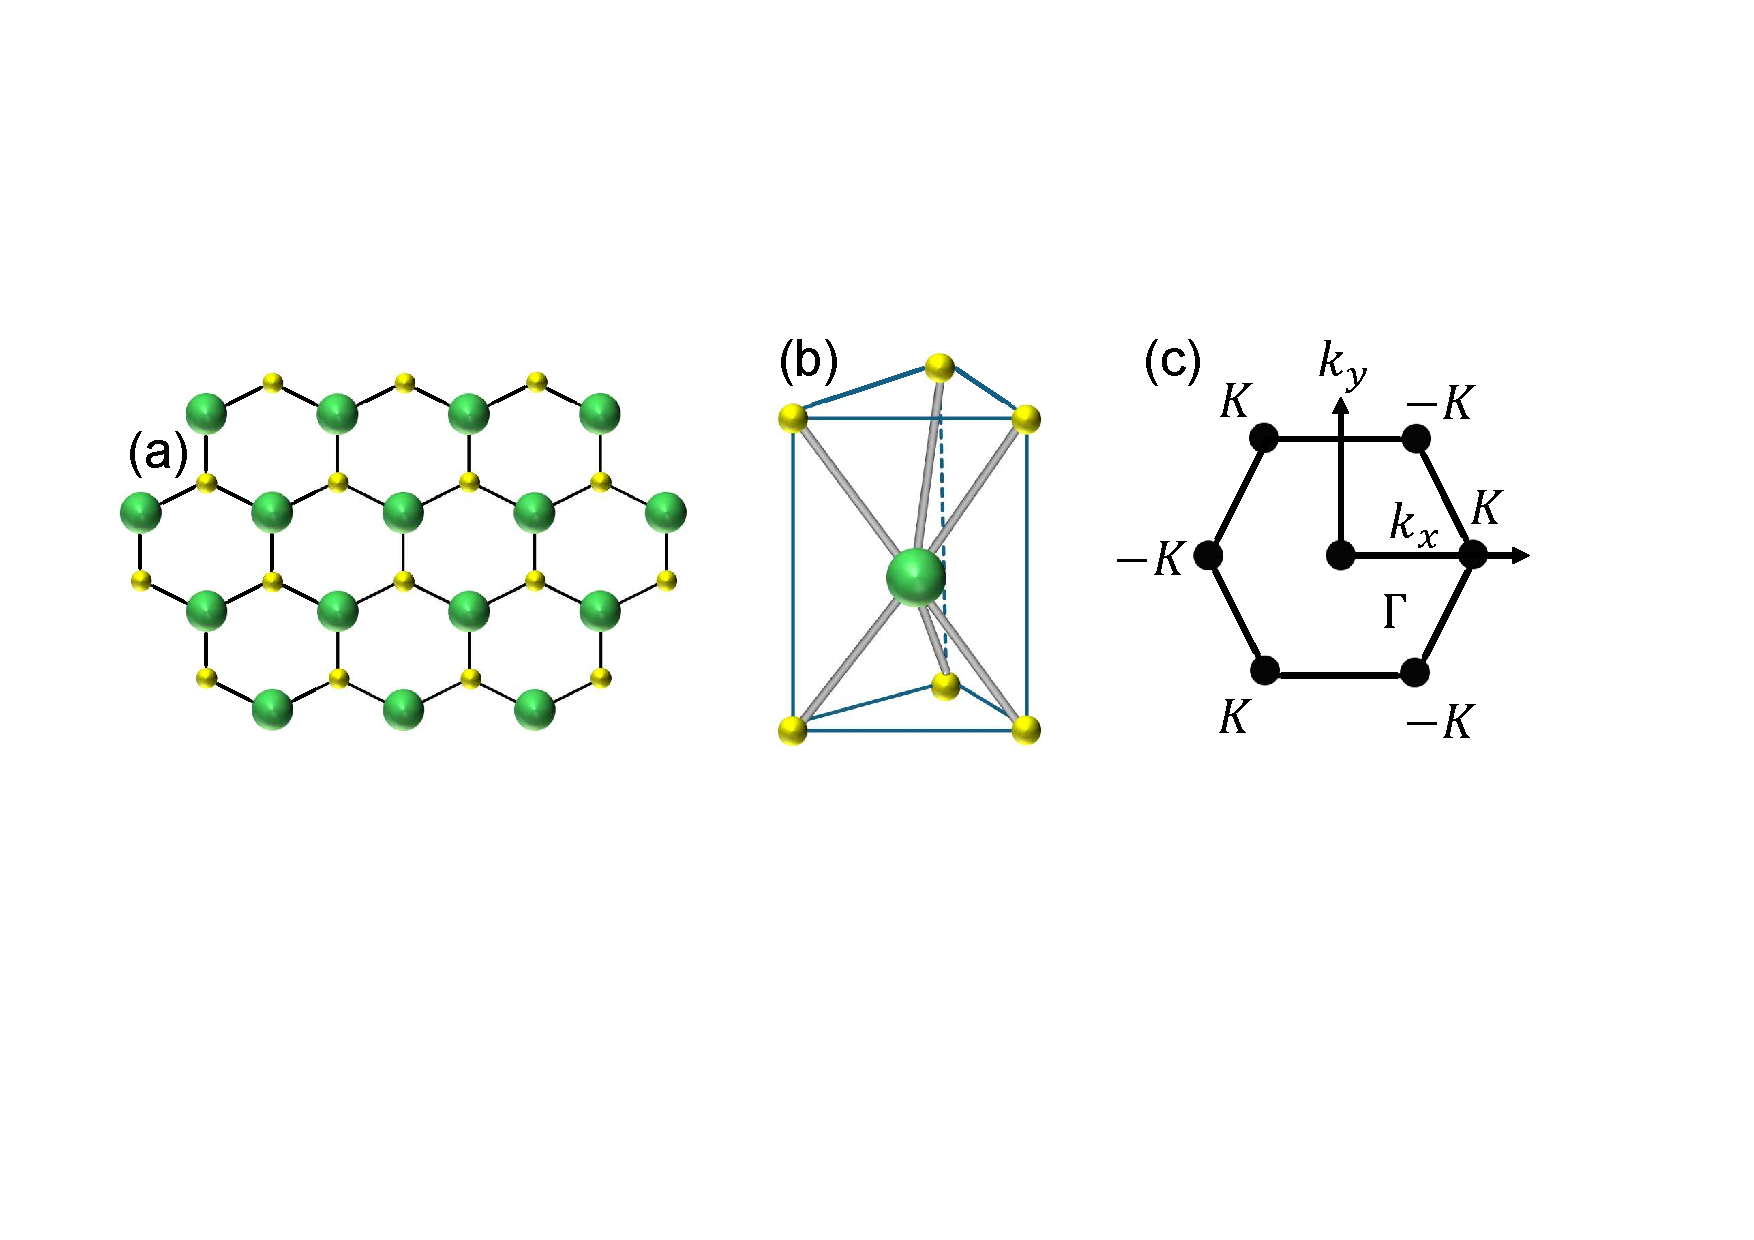
\includegraphics[width=0.5\linewidth,height=0.5\linewidth]{pic/lattice.pdf}
	\caption{\label{fig:Lattice} Top view of monolayer $MX_{2}$. The large sphere is $M$ atom and the small sphere is $X$.}
\end{figure}
Under a uniform magnetic field given by a vector potential $\mathbf{A}(\mathbf{r})$ the single electron Hamiltonian changes into
\begin{align}
	H = \f{\left(-i\hbar \boldsymbol{\nabla} + e \mathbf{A(r)}\right)^{2}}{2m} + U_{0}(\mathbf{r}) + g^{*} \mu_{B} \mathbf{B} \cdot \mathbf{L},
\end{align}
where $\mu_{B} = \f{e\hbar}{2m}$ is Bohr magneton, $g^{*}$ is an effective Landé g-factor, $\mathbf{B} = \boldsymbol{\nabla} \times  \mathbf{A}$ is the uniform magnetic field, and $\mathbf{L}$ is the angular momentum. It is possible to add a phase factor to the tight binding wavefunction
\begin{align}
	\psi_{\lambda,\mathbf{k}} (\mathbf{r}) = \sum_{j=1}^{3} C_{j}^{\lambda} \sum_{\mathbf{R}} e^{i\mathbf{k \cdot R}} e^{i \theta_{\mathbf{R}(\mathbf{r})}} \phi_{j}(\mathbf{r} - \mathbf{R}).
\end{align}
We now have
\begin{align}
	H_{j j'} (\mathbf{k}) = H_{jj'}^{'}(\mathbf{k}) + H_{jj'}^{Z}(\mathbf{k}),
\end{align}
where
\begin{align}
	H_{jj'}(\mathbf{k})
	 & = \sum_{\mathbf{R}} e^{i\mathbf{k \cdot R}} \bra{\phi_{j}(\mathbf{r})} e^{-i \theta_{\mathbf{0}}(\mathbf{r})} \left[\f{(-i\hbar \boldsymbol{\nabla} + e \mathbf{A}(\mathbf{r}))^{2}}{2m} + U_{0}(\mathbf{r}) \right] e^{i \theta_{\mathbf{R}}(\mathbf{r})} \ket{\phi_{j'}(\mathbf{r - R})}\nonumber                  \\
	 & = \sum_{\mathbf{R}} e^{i\mathbf{k \cdot R}} \bra{\phi_{j}(\mathbf{r})} e^{i(\theta_{\mathbf{R}} - \theta_{\mathbf{0}} )} \left[ \f{ \left( -i\hbar \boldsymbol{\nabla} + e \mathbf{A} + \hbar \boldsymbol{\nabla} \theta_{\mathbf{R}} \right)^{2} }{2m} + U_{0}(\mathbf{r}) \right] \ket{\phi_{j'}(\mathbf{r - R})},
\end{align}
and
\begin{align}
	H_{jj'}^{Z}(\mathbf{k})
	 & = g^{*} \mu_{B} \mathbf{B} \cdot \sum_{\mathbf{R}} \bra{\phi_{j}(\mathbf{r})} e^{i(\theta_{\mathbf{R}} - \theta_{\mathbf{0}} )} \mathbf{L} \ket{\phi_{j'}(\mathbf{r - R})}.
\end{align}
By choosing $\theta_{\mathbf{R}} = - \f{e}{\hbar} \int_{\mathbf{R}}^{\mathbf{r}} \mathbf{A(\mathbf{r'})} \cdot d\mathbf{r'}$ as Peierls substitution, the Hamiltonian in Eq. (4) now reads
\begin{align}
	H_{jj'}(\mathbf{k})
	 & = \sum_{\mathbf{R}} e^{i\mathbf{k \cdot R}} \bra{\phi_{j}(\mathbf{r})} e^{ - \frac{ie}{\hbar} \int_{\mathbf{R}}^{\mathbf{r}} \mathbf{A}(\mathbf{r'}) \cdot d\mathbf{r'} + \frac{ie}{\hbar}\int_{\mathbf{0}}^{\mathbf{r}}\mathbf{A(\mathbf{r'})}\cdot d\mathbf{r'} } \left[- \f{\hbar^{2} \boldsymbol{\nabla}^{2}}{2m} + U_{0} (\mathbf{r}) \right] \ket{\phi_{j'}(\mathbf{r - R})} \nonumber \\
	 & = \sum_{\mathbf{R}} e^{i \mathbf{k \cdot R}} e^{\frac{ie}{\hbar} \int_{\mathbf{0}}^{\mathbf{R}} \mathbf{A(\mathbf{r'})} \cdot d \mathbf{r'} } \bra{\phi_{j}(\mathbf{r})} e^{-\frac{ie}{\hbar} \Phi_{\mathbf{R,r,0}}} \left[ -\f{\hbar^{2} \boldsymbol{\nabla}^{2}}{2m} + U_{0} (\mathbf{r}) \right] \ket{\phi_{j'}(\mathbf{r - R})},
\end{align}
where $\Phi_{\mathbf{R,r,0}} = \oint_{\mathbf{R,r,0}} \mathbf{A(\mathbf{r'})} \cdot d\mathbf{r'} $ is the closed loop line intergral of $\mathbf{A}$ along the triangle points $\mathbf{R,r,0}$, and $\int_{\mathbf{0}}^{\mathbf{R}} \mathbf{A(\mathbf{r'})} \cdot d \mathbf{r'}$ is the path intergral along the two points $\mathbf{R,0}$. Besides that, we have used the fact that
\begin{align}
	\int_{\mathbf{R}}^{\mathbf{r}} \mathbf{A(\mathbf{r'})} \cdot d\mathbf{r'} + \int_{\mathbf{r}}^{\mathbf{0}} \mathbf{A(r')} \cdot \mathbf{r'} = \Phi_{\mathbf{R,r,0}} - \int_{\mathbf{0}}^{\mathbf{R}} \mathbf{A(\mathbf{r'})} \cdot d \mathbf{r'}.
\end{align}
We can show that the flux term $\Phi_{\mathbf{R,r,0}}$ is negligibly small \cite{yalcin_2019} by two observations. When $\mathbf{r}$ is far away from the lattice points $\mathbf{R}$ and $\mathbf{0}$, the flux is large but since the atomic orbitals are highly localized at these two lattice points, the value of the hopping term is very small and the whole hopping term goes to zero. While $\mathbf{r}$ is at or near any of these lattice points, the triangle formed is small, and assuming small magnetic field, the flux term $\Phi_{\mathbf{R,r,0}}$ goes to zero, which giving us the Hamiltonian as
\begin{gather}
	H_{jj'}(\mathbf{k})
	= \sum_{\mathbf{R}} e^{i \mathbf{k \cdot R}} e^{\frac{ie}{\hbar} \int_{\mathbf{0}}^{\mathbf{R}} \mathbf{A(\mathbf{r'})} \cdot d \mathbf{r'} } \bra{\phi_{j}(\mathbf{r})} \left[ -\f{\hbar^{2} \boldsymbol{\nabla}^{2}}{2m} + U_{0} (\mathbf{r}) \right] \ket{\phi_{j'}(\mathbf{r - R})},\\
	H_{jj'}^{Z}(\mathbf{k})
	= g^{*} \mu_{B} \mathbf{B} \cdot \sum_{\mathbf{R}} e^{i\mathbf{k\cdot R}} e^{\frac{ie}{\hbar} \int_{\mathbf{0}}^{\mathbf{R}} \mathbf{A(\mathbf{r'})} \cdot d\mathbf{r'} } \bra{\phi_{j}(\mathbf{r})} \mathbf{L} \ket{\phi_{j'}(\mathbf{r - R})}.
\end{gather}
Considering only nearest neighbor(NN) hopping, Eq (2.9) becomes
\begin{equation}
	\begin{aligned}
		H_{\mu\mu'}^{jj'}(\mathbf{k})
		 & = \sum_{\mathbf{R}} e^{\frac{ie}{\hbar}\int_{0}^{\mathbf{R}}A(\mathbf{r'})d\mathbf{r'}}e^{i\mathbf{k\cdot R}} E_{\mu\mu'}^{jj'}(\mathbf{R})                                                                                                                                                   \\
		 & = E_{\mu\mu'}^{jj'}(\mathbf{0}) + e^{\frac{ie}{\hbar}\int_{0}^{\mathbf{R_1}}\mathbf{A(\mathbf{r'})}\cdot d\mathbf{r'}}e^{i\mathbf{k\cdot R_1}} E_{\mu\mu'}^{jj'}(\mathbf{R_1})                                                                                                                \\
		 & + e^{\frac{ie}{\hbar}\int_{0}^{\mathbf{R_2}}\mathbf{A(\mathbf{r'})}\cdot d\mathbf{r'}}e^{i\mathbf{k\cdot R_2}} E_{\mu\mu'}^{jj'}(\mathbf{R_2}) + e^{\frac{ie}{\hbar}\int_{0}^{\mathbf{R_3}}\mathbf{A(\mathbf{r'})}\cdot d\mathbf{r'}}e^{i\mathbf{k\cdot R_3}} E_{\mu\mu'}^{jj'}(\mathbf{R_3}) \\
		 & + e^{\frac{ie}{\hbar}\int_{0}^{\mathbf{R_4}}\mathbf{A(\mathbf{r'})}\cdot d\mathbf{r'}}e^{i\mathbf{k\cdot R_4}} E_{\mu\mu'}^{jj'}(\mathbf{R_4}) + e^{\frac{ie}{\hbar}\int_{0}^{\mathbf{R_5}}\mathbf{A(\mathbf{r'})}\cdot d\mathbf{r'}}e^{i\mathbf{k\cdot R_5}} E_{\mu\mu'}^{jj'}(\mathbf{R_5}) \\
		 & + e^{\frac{ie}{\hbar}\int_{0}^{\mathbf{R_6}}\mathbf{A(\mathbf{r'})}\cdot d\mathbf{r'}}e^{i\mathbf{k\cdot R_6}} E_{\mu\mu'}^{jj'}(\mathbf{R_6}).
	\end{aligned}
\end{equation}

In the presence of a perpendicular magnetic field $\mathbf{B} \hat{z}$ with the vector potential $\vv{A} = (0, Bx, 0)$. For convenience, let us switch to a shorthand notation for these extra terms and define
\begin{gather}
	\theta_{m,n}^{m',n'} \equiv - \f{e}{\hbar} \int_{m,n}^{m',n'} \vv{A} \cdot d\mathbf{r}.
\end{gather}
\begin{figure}[H]
	\centering
	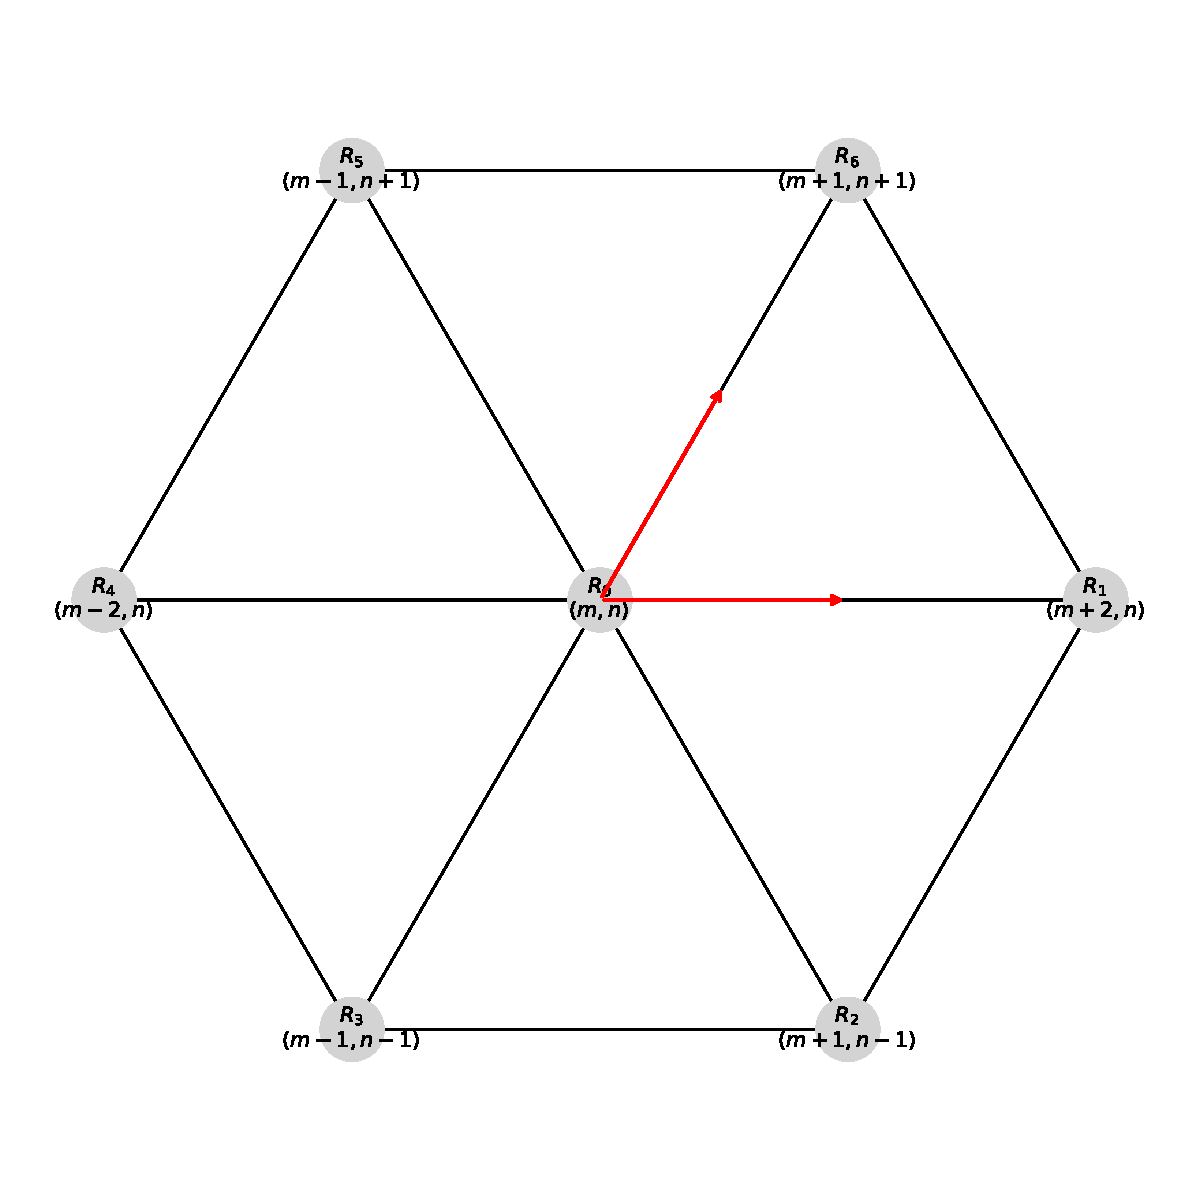
\includegraphics[width=0.5\linewidth,height=0.5\linewidth]{pic/siteindice.pdf}
	\caption{\label{fig:site index} Site index}
\end{figure}
With the given Landau gauge, the line intergral $\int \vv{A} \cdot d\mathbf{r}$ is evaluated to $\int Bx dy$. Let us now express the Hamiltonian from the zero-field are given by \cite{PhysRevB.88.085433} with the transform hopping parameters, noting that the NN coordinates are $x = \frac{ma}{2}(m = \pm 1, \pm 2)$ and $y = \frac{na\sqrt{3}}{2}(n = 0,\pm 1)$, $a$ being the lattice constant, are shown in \hyperref[fig:site index]{Fig (2.2)}. Since $dy = 0$ along the $x$ direction, $\theta_{m,n}^{m \pm 2, n} = 0$, and using $ansatz$ $x = \frac{ma}{2}$ for lattice site, the $\theta_{m,n}^{m',n'}$ can be written as
\begin{gather}
	\theta_{m,n}^{m',n'} =
	\begin{cases}
		0                                                         & \quad m' = m \pm 2, n' = n     \\
		\pm \frac{e}{\hbar} \frac{B a^{2} \sqrt{3}}{2} (m + 1 /2) & \quad m' = m + 1, n' = n \pm 1 \\
		\pm \frac{e}{\hbar} \frac{B a^{2} \sqrt{3}}{2} (m - 1 /2) & \quad m' = m - 1, n' = n \pm 1 \\
	\end{cases}
\end{gather}
Identifying $\frac{B a^{2} \sqrt{3}}{2}$ as the magnetic flux $\Phi$ passing through per unit cell and $h / e$ as the flux quantum $\Phi_{0}$, then we have
\begin{equation}
	\begin{aligned}
		H_{\mu\mu'}^{jj'}(\mathbf{k})
		 & = E_{\mu\mu'}^{jj'}(\mathbf{0}) + e^{i\theta_{m,n}^{m',n'} }e^{i \mathbf{k} \cdot \mathbf{R}_{1}} E_{\mu\mu'}^{jj'}(\mathbf{R}_{1}) + e^{i\theta_{m,n}^{m',n'} } e^{i \mathbf{k} \cdot \mathbf{R}_{2}} E_{\mu\mu'}^{jj'}(\mathbf{R}_{2}) \\
		 & + e^{i\theta_{m,n}^{m',n'} } e^{i \mathbf{k} \cdot \mathbf{R}_{3}} E_{\mu\mu'}^{jj'}(\mathbf{R}_{3}) + e^{i\theta_{m,n}^{m',n'} }e^{i \mathbf{k} \cdot \mathbf{R}_{4}} E_{\mu\mu'}^{jj'}(\mathbf{R}_{4})                                 \\
		 & + e^{i\theta_{m,n}^{m',n'} } e^{i \mathbf{k} \cdot \mathbf{R}_{5}} E_{\mu\mu'}^{jj'}(\mathbf{R}_{5}) + e^{i\theta_{m,n}^{m',n'} }e^{i \mathbf{k} \cdot \mathbf{R}_{6}} E_{\mu\mu'}^{jj'}(\mathbf{R}_{6}).
	\end{aligned}
\end{equation}
The Hamiltonian depends on the site index $m$ and does not invariant under the translation of a lattice vector along the $x$ axis. In order to restore this invariance, we can look at the case where the ratio of magnetic flux and flux quanta is a rational number $\Phi / \Phi_{0} = p / q$. This mean, we have expand the unit cell in the $x$ direction, the Hamiltonian becomes invariant under translational, allowing us to define what we will call the magnetic unit cell, which is consisting of $q$ $M$-atoms %Hinh. 
We define a new basis set of $3q$ atomic orbitals $\phi_{\mu}^{j} (x,y) = \phi_{\mu}^{j} (ma/2,y)$ where $m = 1,2,...q$. Note that
\begin{gather}
	\begin{cases}
		e^{i k_{x} a} \phi_{\mu}^{j} \left(m \frac{a}{2},y\right) = \phi_{\mu}^{j} \left((m+2)\frac{a}{2},y\right)            & ;\;  e^{-i k_{x} a} \phi_{\mu}^{j} \left(m\frac{a}{2},y\right) = \phi_{\mu}^{j} \left((m-2)\frac{a}{2},y\right)           \\
		e^{i k_{x} \frac{a}{2}} \phi_{\mu}^{j} \left(m \frac{a}{2},y\right) = \phi_{\mu}^{j} \left((m+1)\frac{a}{2},y\right) & ;\;  e^{-i k_{x} \frac{a}{2}} \phi_{\mu}^{j} \left(m\frac{a}{2},y\right) = \phi_{\mu}^{j} \left((m-1)\frac{a}{2},y\right)
	\end{cases}
\end{gather}
Consequently the Hamiltonian matrix in the new basis is written as
\begin{equation}
	\begin{aligned}
		H_{\mu\mu'}^{jj'}(\mathbf{k})
		 & = E_{\mu\mu'}^{jj'}(\mathbf{0}) + e^{i\theta_{m,n}^{m',n'}} E_{\mu\mu'}^{jj'}(\mathbf{R}_{1}) \delta_{m,m+2}\delta_{n,n} + e^{i\theta_{m,n}^{m',n'}} E_{\mu\mu'}^{jj'}(\mathbf{R}_{2}) \delta_{m,m+1} \delta_{n,n - 1} \\
		 & + e^{i\theta_{m,n}^{m',n'}} E_{\mu\mu'}^{jj'}(\mathbf{R}_{3}) \delta_{m,m - 1} \delta_{n,n - 1} + e^{i\theta_{m,n}^{m',n'}} E_{\mu\mu'}^{jj'}(\mathbf{R}_{4}) \delta_{m,m + 2} \delta_{n,n}                            \\
		 & + e^{i\theta_{m,n}^{m',n'}} E_{\mu\mu'}^{jj'}(\mathbf{R}_{5}) \delta_{m,m - 1} \delta_{n,n + 1} + e^{i\theta_{m,n}^{m',n'}} E_{\mu\mu'}^{jj'}(\mathbf{R}_{6}) \delta_{m,m + 1} \delta_{n,n + 1}.
	\end{aligned}
\end{equation}
Now, for given flux ratio $p/q$, only the $q$ determines the periodicity of the magnetic cell assuming $p$ and $q$ are mutually prime numbers. When we plot the band energies while varying the $p$, we obtain the famous Hofstadter butterfly \cite{PhysRevB.14.2239}, a complex fractal structure as seen in Fig. 2.3. This structure is generated at the $K = (\frac{4\pi}{3a},0)$ k-point. This fractal spectrum is a result of two competing effects, lattice periodicity and magnectic unit cell periodicity enforced by the presence of the magnetic field. Eq. 2.16 give the following matrix which must be diagonalized to obtain the energy eigenvalues.

The magnetic field enters the TB Hamiltonian only through the fraction $p/q$, which is the magnetic flux through the primitive unit cell of the lattice.In general, as the lattice geometry evolves, the area of the primitive unit cell changes $(m + 1/2)$ times

An alternative approach to the derivation of the Hamiltonian under an uniform magnetic field is given in \hyperref[appendix b]{Appendix B}.
\begin{figure*}[htb]
	\centering
	\begin{subfigure}[b]{0.495\textwidth}
		\centering
		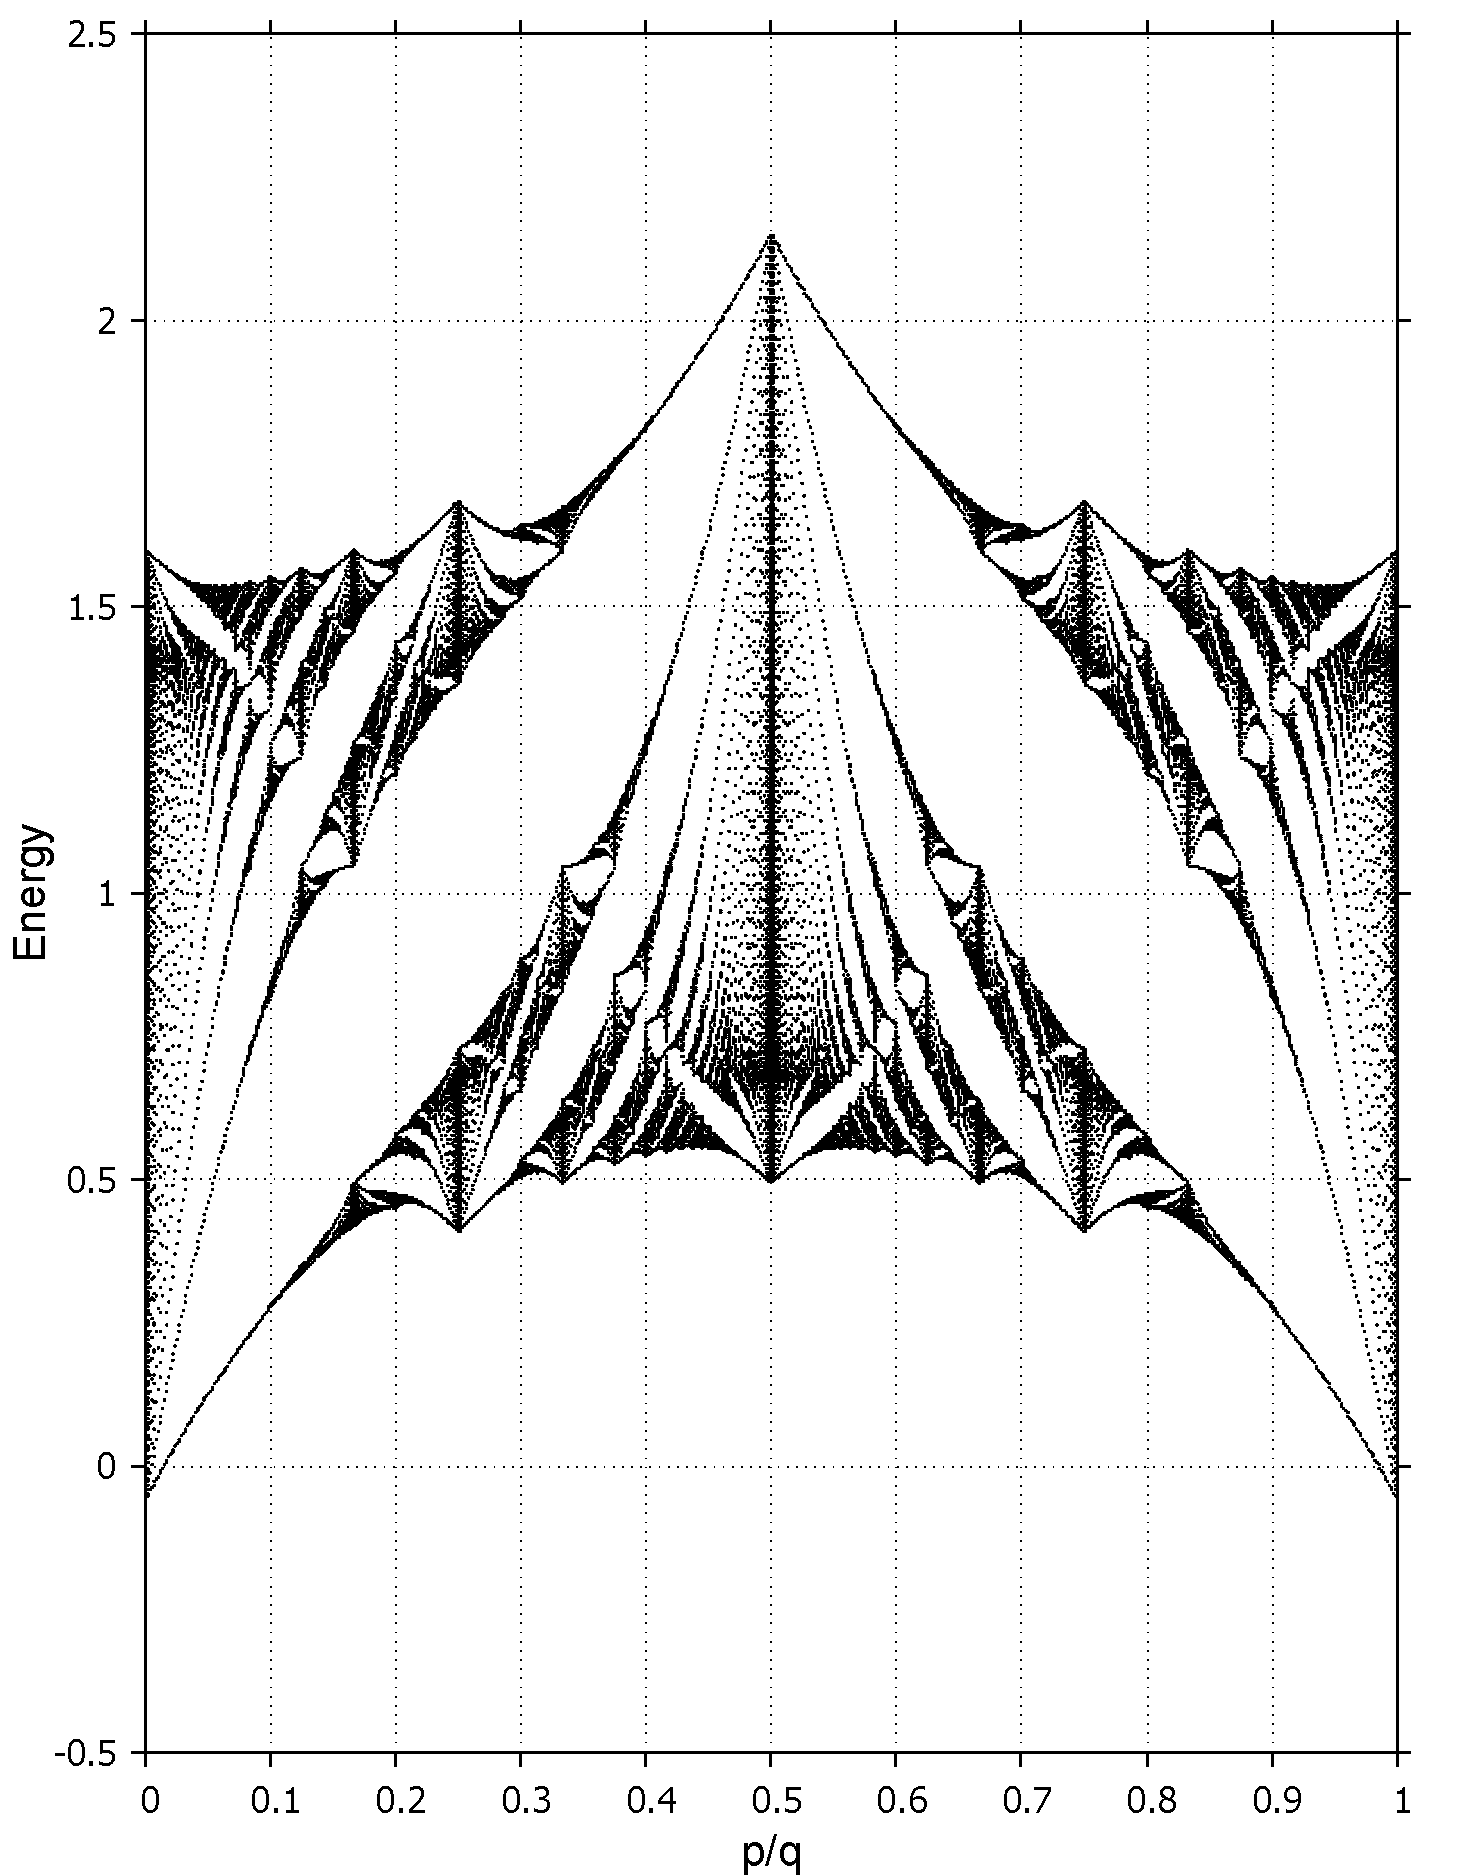
\includegraphics[width=0.85\textwidth,height=1.2\linewidth]{pic/h0_tam giac_q_797.png}
		\label{fig:3 band}
	\end{subfigure}
	\begin{subfigure}[b]{0.495\textwidth}
		\centering
		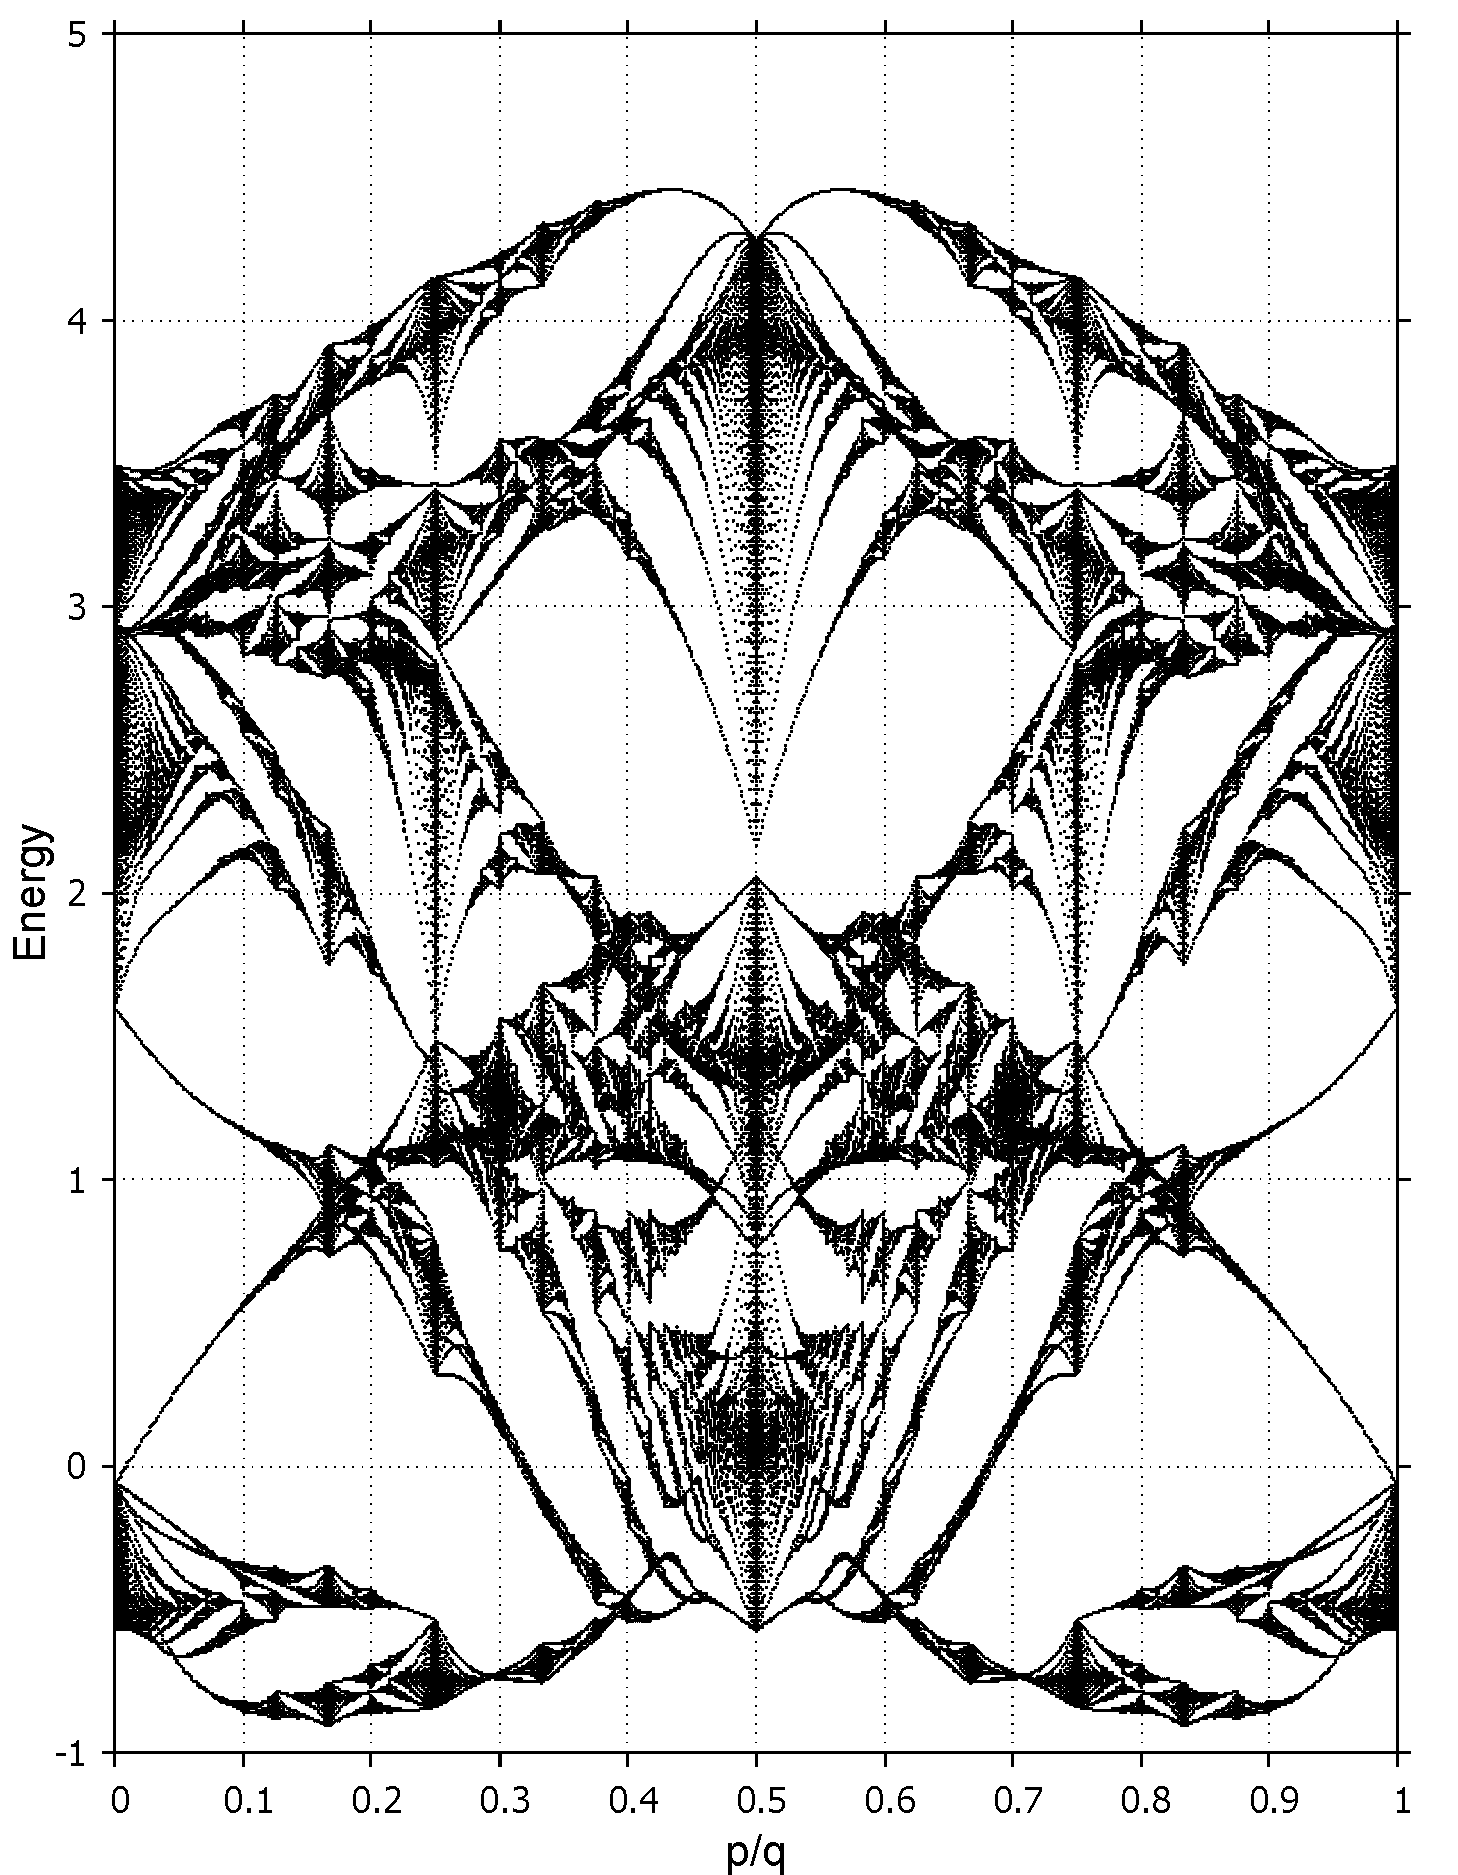
\includegraphics[width=0.85\textwidth,height=1.2\linewidth]{pic/3band_gnuplot_q_797.png}
		\label{fig:1 band}
	\end{subfigure}
	\caption{
		Hofstadter’s butterfly for one band $\ket{dz} \equiv \ket{\phi_{1}^{1}(x,y)}$(left) and all band(right) with $q = 797$ and vary $p$  from 1 to $q$ with field strength $B_{0} = 4.6928 \times 10^{4}$ T.
	}
\end{figure*}
\section{Spin-orbit coupling}
Due to the heavy mass of the transistion-metal $M$ atom, its spin orbit coupling(SOC) can be large. For the sake of simplicity, only the on-site contribution, namely, the $\mathbf{L \cdot S}$ term from $M$ atoms. Using the bases $\left\{\ket{d_{z^{2}},\uparrow},\ket{d_{xy},\uparrow},\ket{d_{x^{2} - y^{2}},\uparrow},\ket{d_{z^{2}},\downarrow},\ket{d_{xy},\downarrow},\ket{d_{x^{2} - y^{2} },\downarrow}\right\}$, we get the SOC contribution to the Hamiltonian as
\begin{gather}
	H^{'}
	= \lambda \mathbf{L \cdot S}
	= \f{\lambda}{2}
	\begin{pNiceMatrix}
		L_{z} & 0      \\
		0     & -L_{z}
	\end{pNiceMatrix},
\end{gather}
in which
\begin{gather}
	L_{z}
	=
	\begin{pNiceMatrix}
		0 & 0   & 0  \\
		0 & 0   & 2i \\
		0 & -2i & 0
	\end{pNiceMatrix}
\end{gather}
is the matrix of $\hat{L}_{z}$($z$ component of the orbital angular momentum) in bases of $d_{z^{2}},d_{xy},d_{x^{2} - y^{2}}$ and $\lambda$ is characterized the strength of the SOC. Noting that, under the three bases, the matrix elements of $\hat{L}_{x}$ and $\hat{L}_{y}$ are all zeros. There for the Hamiltonian for the magnetic unit cell with the SOC as follows
\begin{equation}
	\begin{aligned}
		H_{\text{SOC}}(\mathbf{k})S
		 & = \mathbf{I}_{2} \otimes H_{0}(\mathbf{k}) + H'
	\end{aligned}
\end{equation}



\section{Landau levels}
In solid-state physics, the behavior of electrons in magnetic fields is usually introduced by using the Hamiltonian
\begin{gather}
	H = \f{\mathbf{p} + e \mathbf{A}(\mathbf{r})^{2}}{2m} .
\end{gather}

\begin{gather}
	E = \left(n + 1/2\right) \hbar \omega_{c}
\end{gather}
and the energy eigenfunctions are known as Landau levels.

This treatment is for free electrons, \cite{10.1119/1.1615568} but near the bottom of the two-dimensional tigh-binding band of TMD, the energy is approximately free-electron-like by Taylor expanding to second order of $\mathbf{k}$ 
\begin{equation}
	\begin{aligned}
		E(\mathbf{k})
		 & \approx 2 t_{0} \left[1 - \frac{a^{2} k_{x}^{2}}{2} + 2\left(1 - \f{a^{2} k_{x}^{2}}{8}\right)\left(1 - \f{3a^{2} k_{y}^{2}}{8}\right)\right] \\
		 & = t_{0} \f{3}{16} \left(32 + a^{4} k_{x}^{2} k_{y}^{2}\right) - t_{0} \f{3}{2} a^{2}(k_{x}^{2} + k_{y}^{2}) ,
	\end{aligned}
\end{equation}
the first term $a^{2}$ is negligibly small and another can be treated like constant, then we have
\begin{gather}
	E(\mathbf{k})
	\approx 6 t_{0} - \f{\hbar^{2}}{2m} (k_{x}^{2} + k_{y}^{2}),
\end{gather}
where $m^{*} = \f{\hbar^{2}}{(3t_{0}a^{2} / 4) }$ is the effective mass. Hence, the cyclotron frequency is
\begin{gather}
	\omega_{c} = \f{eB}{m^{*}} = \f{\sqrt{3}}{2} t_{0} \f{p}{q},
\end{gather}
and therefore the Landau levels near the bottom of the band $\ket{d_{z^{2}}}$ can be written as
\begin{gather}
	E(\mathbf{k}) = t_{0} \left(6 - \sqrt{3} \f{p}{q}( n + 1 /2)\right),
\end{gather}
in linear order of an uniform-flux, where $n$ is Landau index.
\begin{figure*}[htb]
	\centering
	\begin{subfigure}[b]{0.49\textwidth}
		\centering
		{\caption{}\label{fig:3 landau level 1}}
		{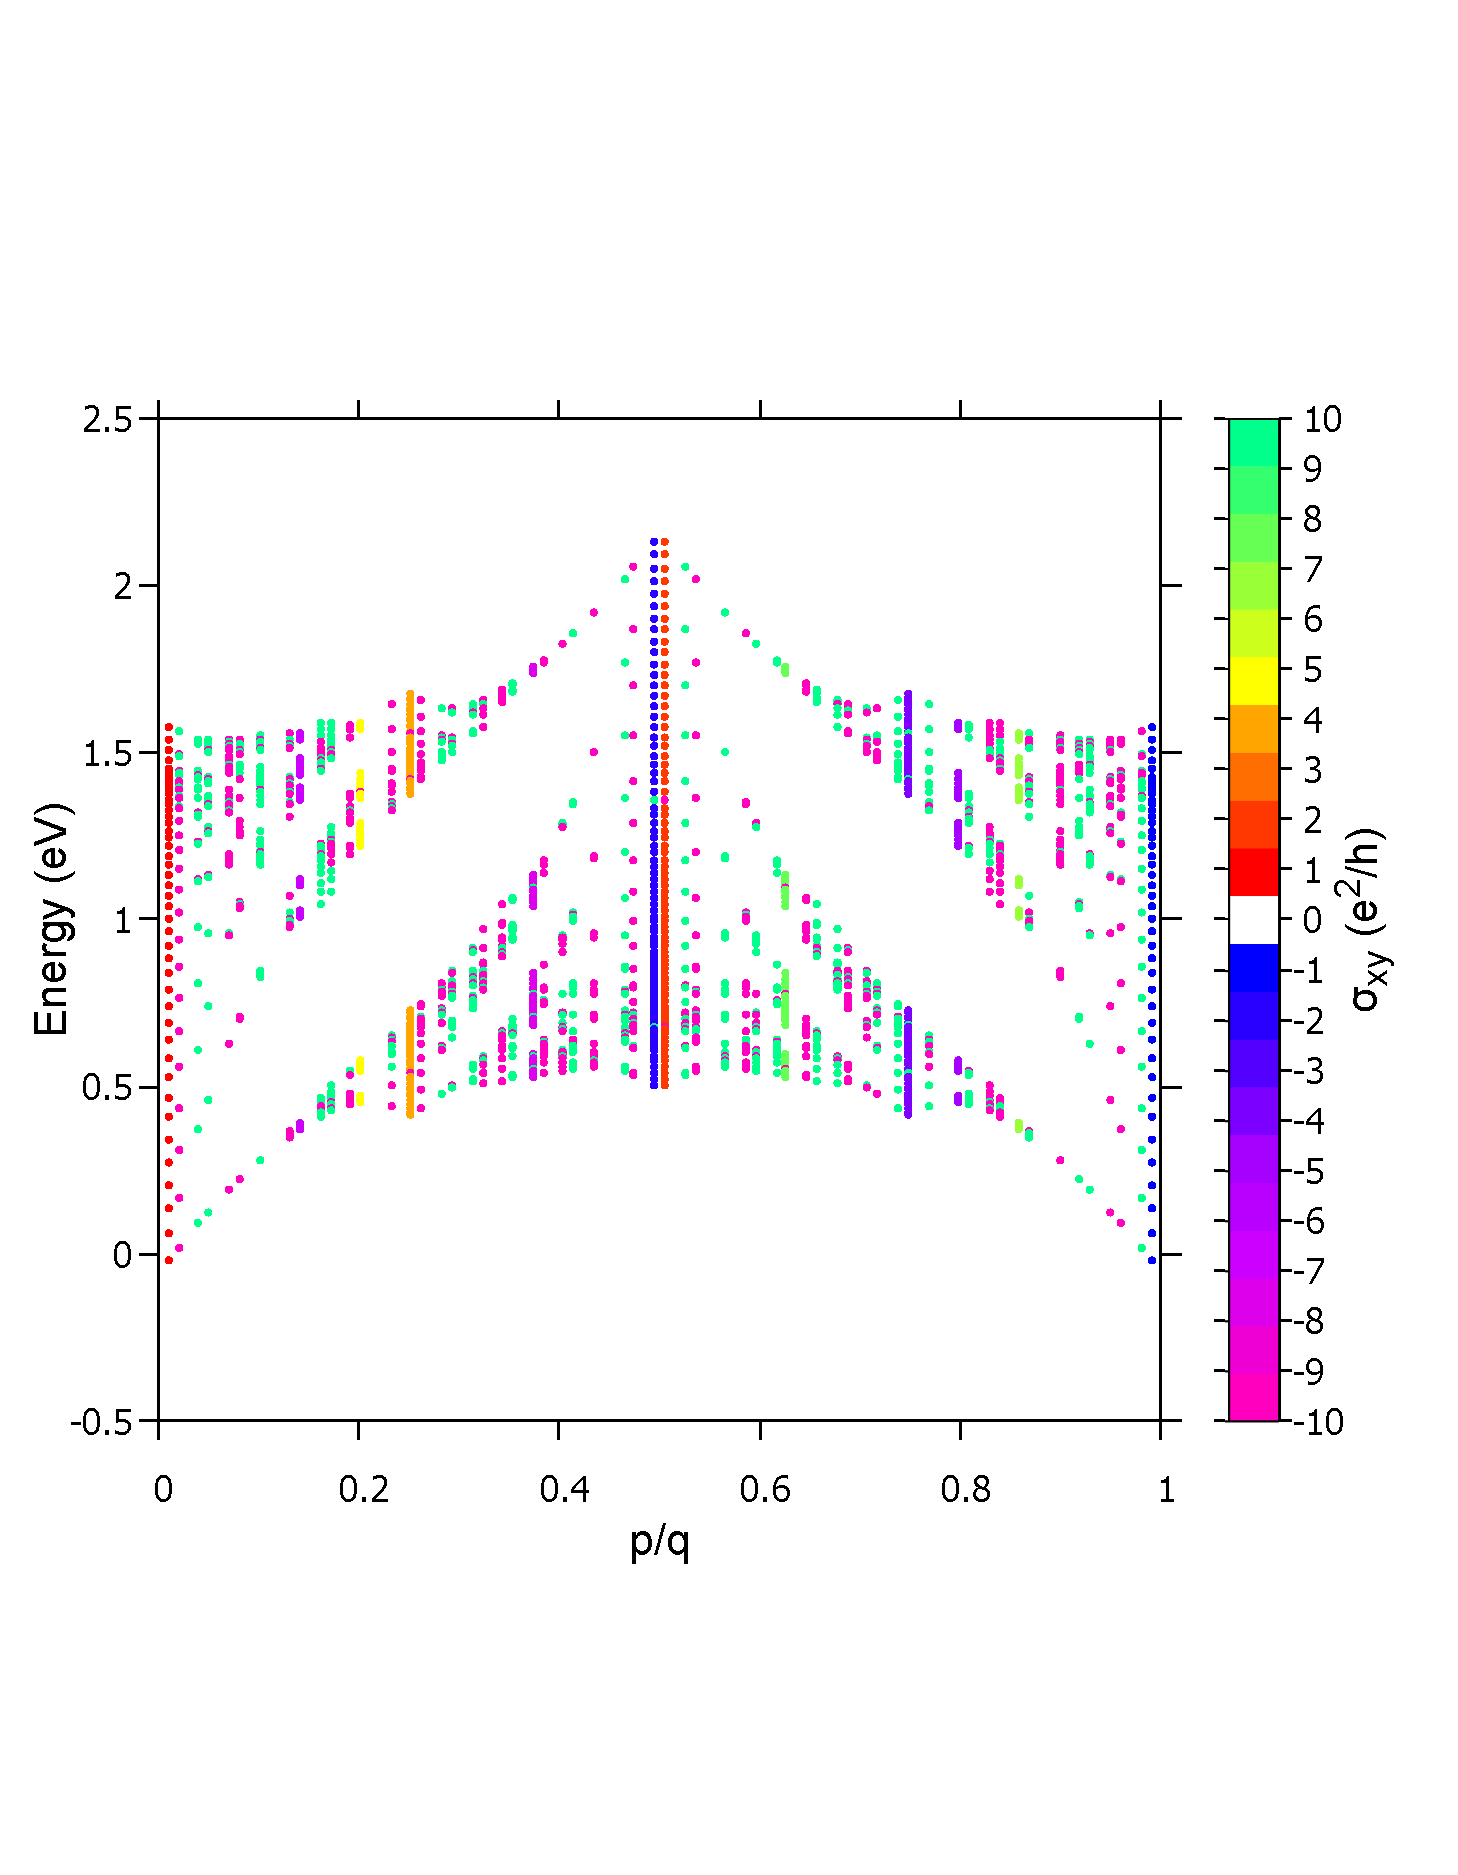
\includegraphics[width=0.85\textwidth,height=1.2\linewidth]{pic/test.png}}
	\end{subfigure}
	\begin{subfigure}[b]{0.49\textwidth}
		\centering
		\caption{}\label{fig:1 landau level 2}
		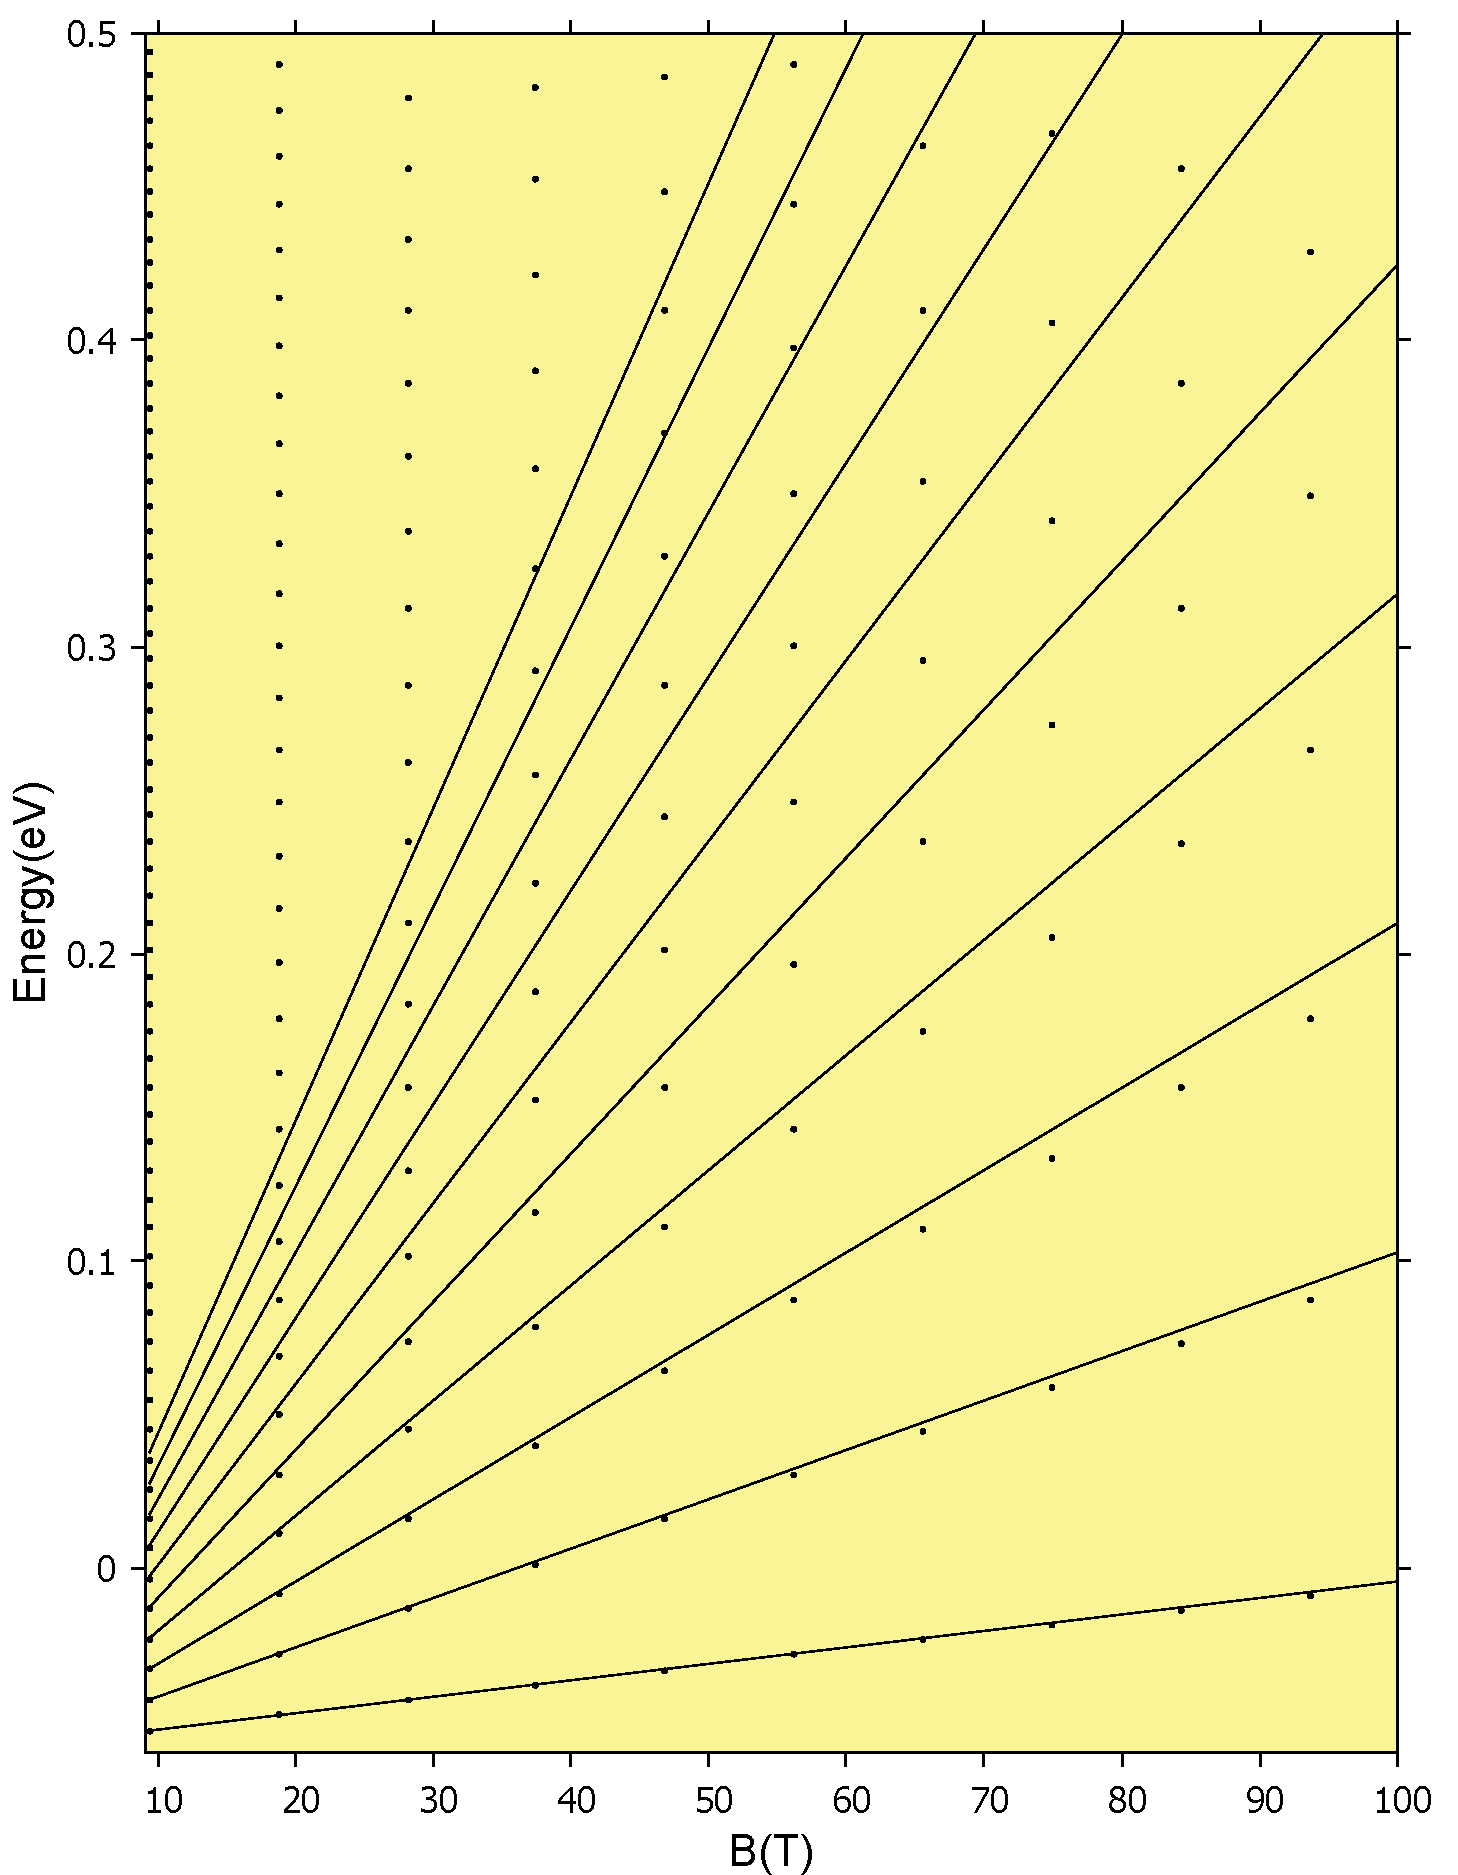
\includegraphics[width=0.85\textwidth,height=1.2\linewidth]{pic/landaulevel_h0_q_797.pdf}
	\end{subfigure}
	\caption{
		(a) Same plot as Fig 2.3 but we consider a small area and (b) is the Landau fan diagram show for the first $n = 10$ levels near the bottom of the conduction band for a magnetic field up to $B = 100\; T$.
	}
\end{figure*}

In Fig 2.4 we compare the spectrum of a small section of triangular lattice with $p / q = 1 / 797$. With the fan of Landau levels given by Eq.(2.26) plotted in Fig 2.4(b). The fan of Landau levels can be clearly seen emergin from the partern in Fig 2.4(a). It is this fan of Landau levels that responsiblee for the de Haas-van Alphen and Shubnikov-de Haas effects. \cite{Shoenberg_1984,singleton2001band,blundell2001magnetism,kittel1987quantum} The Landau levels are all close to being linear in $B$, resulting from the magnetic quantization of parabolic bands at $B = 0$. In our model study, Landau levels can be classified into specific groups. In each group, each levels can be further labeled by a Landau index $n$. Figure 2.4 displays a blowup of the low uniform magnetic region and the LLs as a function of $\Phi / \Phi_{0}$ \cite{Li_2011}



\chapter{DISCUSSION AND FUTURE WORK}






\nocite{*}
\renewcommand{\bibname}{REFERENCES}
\bibliographystyle{unsrt}
\bibliography{refs}
\appendix
\renewcommand{\chaptername}{Appendix}
\chapter{Construct matrix}
In Ref. \cite{PhysRevB.88.085433},G-B Liu $et \; al$. contructed 


\chapter{Harper's equation} \label{appendix b} 
Let us consider the case of hexagonal lattice with $\ket{d_{z^{2}}}$ band as a basis under an uniform magneticc field given by the Landau gauge $\vv{A} = (0, Bx,0)$. Given
\begin{equation}
	\begin{aligned}
		h_0
		 & = 2 t_0 \left(\cos2\alpha + 2\cos\alpha \cos\beta\right) + \epsilon_1                                                                                                                                                                                                                                                                                                                                                                                                             \\
		 & = 2t_{0} \left[ \cos(k_x a) + 2 \cos \left(\f{k_x a}{2}\right) \cos \left(\f{\sqrt{3}k_y a}{2}\right) \right] + \epsilon_1                                                                                                                                                                                                                                                                                                                                                        \\
		 & = 2t_{0} \left\{ \cos(k_x a) + \cos\left[\left( k_{x} + \sqrt{3} k_{y} \right)\frac{a}{2}\right] + \cos\left[\left( k_{x} - \sqrt{3} k_{y} \right)\frac{a}{2}\right]\right\} + \epsilon_1                                                                                                                                                                                                                                                                                                                                                        \\
		 & = 2t_{0} \Biggl\{ \cos(p_{x}\f{a}{\hbar}) + \cos \left[\left(p_{x} + \sqrt{3} e B x + \sqrt{3} p_{y}\right)\frac{a}{2\hbar}\right] \\
		 &+ \cos \left[\left(p_{x} - \sqrt{3} e B x - \sqrt{3} p_{y}\right)\frac{a}{2\hbar}\right] \Biggr\} + \epsilon_1                                                                                                                                                                                                                                                                                                  \\
		 & = t_{0} \biggl[e^{i p_{x}\frac{a}{\hbar}} + e^{-ip_{x}\frac{a}{\hbar}} + e^{i(p_{x} + \sqrt{3} eBx + \sqrt{3} p_{y} ) a / 2\hbar} + e^{-i(p_{x} + \sqrt{3} eBx + \sqrt{3} p_{y} ) a / 2\hbar} \\
		 &+ e^{i(p_{x} - \sqrt{3} eBx - \sqrt{3} p_{y} ) a / 2\hbar} + e^{-i(p_{x} - \sqrt{3} eBx - \sqrt{3} p_{y} ) a / 2\hbar} \biggr] + \epsilon_1.
	\end{aligned}
\end{equation}
We replaced $\hbar k$ in the above function by the operators $\vv{p} - e \vv{A} / c$ in order to create an operator out of $h_{0}$. When this substitution is made, the Hamiltonian element is seen to contain translation operators $\exp[a p_{x} / \hbar],\exp[a \sqrt{3} p_{y} / (2\hbar)]$. Depending on the gauge chosen, there are, in addition, certain phase factors dependent on the magnetic field strength, which multiply the translation operators. The Landau gauge was $\vv{A} = (0,Bx,0)$ was chosen, then only the translation along $y$ are multiplied by phases. \cite{PhysRevB.14.2239}
Applying the BCH's formula and taking to account the commutation relation $\left[x,p_{x}\right] = i \hbar$
\begin{equation}
	\begin{aligned}
		e^{\pm i(p_{x} + \sqrt{3} e B x) a / 2\hbar} 
		&= e^{\pm i p_{x} a / 2 \hbar} e^{\pm i\sqrt{3} e B x a / 2 \hbar} e^{-\frac{1}{2} \left[\pm i p_{x}, \pm i \sqrt{3} e B x\right] a^{2} / 2 \hbar^{2}} \\
		&= e^{\pm i p_{x} a / 2 \hbar} e^{\pm i\sqrt{3} e B x a / 2 \hbar} e^{\mp i \sqrt{3} e B a^{2} / 8 \hbar}
	\end{aligned}
\end{equation}
Substituting $x = \f{ma}{2}$ into (B.2), this leads to
\begin{gather}
	e^{\pm i(p_{x} + \sqrt{3} e B x) a / 2\hbar}
	= e^{\pm i p_{x} a / 2 \hbar} e^{\pm i\sqrt{3} e B (m + 1 /2) a / 4 \hbar}
\end{gather}
And 
\begin{equation}
	\begin{aligned}
		e^{\pm i(p_{x} - \sqrt{3} e B x) a / 2\hbar} 
		&= e^{\pm i p_{x} a / 2 \hbar} e^{\mp i\sqrt{3} e B x a / 2 \hbar} e^{-\frac{1}{2} \left[\pm i p_{x}, \mp i \sqrt{3} e B x\right] a^{2} / 2 \hbar^{2}} \\
		&= e^{\pm i p_{x} a / 2 \hbar} e^{\mp i\sqrt{3} e B x a / 2 \hbar} e^{\mp i \sqrt{3} e B a^{2} / 8 \hbar}
	\end{aligned}
\end{equation}
Substituting $x = \f{ma}{2}$ into (B.4), this leads to
\begin{gather}
	e^{\pm i(p_{x} - \sqrt{3} e B x) a / 2\hbar}
	= e^{\pm i p_{x} a / 2 \hbar} e^{\mp i\sqrt{3} e B (m - 1 /2) a^{2} / 4 \hbar}
\end{gather}
The operators $e^{\pm i p_{x} a / 2 \hbar}, e^{\pm i p_{y} \sqrt{3}a / 2 \hbar}$ can be regconized as translational operators, we can rewrite (B.1) as
The time-indepentdent Schr\"{o}dinger's equation now becomes
\begin{equation}
	\begin{aligned}
 		& t_{0} \varphi_{1} (x + a,y) + t_{0}\varphi_{1} (x - a,y) + t_{0}\varphi_{1} (x + \frac{a}{2},y + \frac{a\sqrt{3}}{2}) e^{\frac{ie}{\hbar}B(m + 1 /2) \frac{a^{2}\sqrt{3}}{4}} \\
		+ & t_{0} \varphi_{1} (x + \frac{a}{2},y - \frac{a\sqrt{3}}{2}) e^{-\frac{ie}{\hbar}B(m + 1/2) \frac{a^{2}\sqrt{3}}{4}} + t_{0} \varphi_{1} (x - \frac{a}{2},y + \frac{a\sqrt{3}}{2}) e^{\frac{ie}{\hbar}B(m + 1/2) \frac{a^{2}\sqrt{3}}{4}} \\
		+ & t_{0} \varphi_{1} (x - \frac{a}{2},y - \frac{a\sqrt{3}}{2}) e^{-\frac{ie}{\hbar}B(m - 1/2) \frac{a^{2}\sqrt{3}}{4}} + \epsilon_{1} \varphi_{1}(x,y) = E_{1} \varphi_{0}(x,y),
	\end{aligned}
\end{equation}
for the sake of simplicity let us define $\varphi_{0} \equiv \ket{d_{z^{2}}}$.\\
%We have established in Section 2.2 that when translated by a lattice vector $\mathbf{R}$, the wavefuntion for an electron in a periodic lattice picks up a phase correspondingly. This lets us define
%\begin{gather}
%	\varphi(x \pm a,y) = e^{\pm i k_{x} a} \varphi(x,y), \\ 
%	\varphi(x \pm \f{a}{2},y \pm \f{a\sqrt{3}}{2}) = e^{\pm i k_{x} \frac{a}{2}} e^{\pm i k_{y} \frac{a\sqrt{3}}{2}} \varphi(x,y).
%\end{gather}
%Substituting $x = m \f{a}{2}$ and $y = n \f{a\sqrt{3}}{2}$ for the given hexagonal lattice, we can express the time-indepentdent Schr\"{o}dinger equation as 
%\begin{equation}
%	\begin{aligned}
%		&t_{0} \varphi_{0}(m + 2, n) + t_{0} \varphi_{0}(m - 2, n) + t_{0} \varphi_{0}(m + 1, n + 1) e^{\frac{ie}{\hbar}Bm \frac{a^{2}\sqrt{3}}{4}} \\
%		+& t_{0} \varphi_{0}(m + 1, n - 1) e^{-\frac{ie}{\hbar}Bm \frac{a^{2}\sqrt{3}}{4}} + t_{0} \varphi_{0}(m - 1, n + 1) e^{\frac{ie}{\hbar}Bm \frac{a^{2}\sqrt{3}}{4}} \\
%		+& t_{0} \varphi_{0}(m - 1, n - 1) e^{-\frac{ie}{\hbar}Bm \frac{a^{2}\sqrt{3}}{4}} + \epsilon_{1} \varphi_{0}(m,n) = E_{1} \varphi_{0}(m,n).
%	\end{aligned}
%\end{equation}
It is reasonable to assume planewave behavior in the $y$ direction, since the coefficents in the above equation only involve $x$. Therefore, we can assume the partial solution for $y$ to be in the form 
\begin{gather}
	\varphi(\frac{ma}{2},\frac{na\sqrt{3}}{2}) = e^{i k_{y} n \frac{a\sqrt{3}}{2}} G(m),
\end{gather}
which reduces (B.6) to
\begin{equation}
	\begin{aligned}
		&t_{0} \varphi_{0}(m + 2) + t_{0} \varphi_{0}(m - 2) + t_{0} \varphi_{0}(m + 1) e^{2 i \pi (m + 1 /2) p/ q} e^{i k_{y} a\sqrt{3} / 2} \\
		 +& t_{0} \varphi_{0}(m + 1) e^{-2 i \pi (m + 1 /2) p/ q} e^{-i k_{y} a\sqrt{3} / 2} + t_{0} \varphi_{0}(m - 1) e^{2 i \pi (m - 1 /2) p/ q} e^{i k_{y} a\sqrt{3} / 2} \\
		+& t_{0} \varphi_{0}(m - 1) e^{-2 i \pi (m - 1 /2) p/ q} e^{-i k_{y} a\sqrt{3} / 2} + \epsilon_{1} \varphi_{0}(m) = E_{1} \varphi_{0}(m),
	\end{aligned}
\end{equation}
this is equivalent to Eq. 2.16 we have mentioned in Section 2.2. Equation B.7 is sometimes called ``Harper's equation''. \cite{harper1955general} Since different $m$ values give different equations, one reaches a unique set of equations when $\Phi / \Phi_{0}$ is a rational number $p / q$ and $m$ goes through $q$ different values, essentially resulting in the Hamiltonian matrix written for a magnetic unit cell enlarged in $x$ direction $q$ times.

\chapter{Phase factor}
\begin{equation}
	\begin{aligned}
		H_{\mu\mu'}^{jj'}(\mathbf{k})
		& = \sum_{\mathbf{R}} e^{\frac{ie}{\hbar}\int_{0}^{\mathbf{R}}A(\mathbf{r'})d\mathbf{r'}}e^{i\mathbf{k\cdot R}} E_{\mu\mu'}^{jj'}(\mathbf{R})                                                                                                                                                   \\
		& = E_{\mu\mu'}^{jj'}(\mathbf{0}) + e^{\frac{ie}{\hbar}\int_{0}^{\mathbf{R_1}}\mathbf{A(\mathbf{r'})}\cdot d\mathbf{r'}}e^{i\mathbf{k\cdot R_1}} E_{\mu\mu'}^{jj'}(\mathbf{R_1})                                                                                                                \\
		& + e^{\frac{ie}{\hbar}\int_{0}^{\mathbf{R_2}}\mathbf{A(\mathbf{r'})}\cdot d\mathbf{r'}}e^{i\mathbf{k\cdot R_2}} E_{\mu\mu'}^{jj'}(\mathbf{R_2}) + e^{\frac{ie}{\hbar}\int_{0}^{\mathbf{R_3}}\mathbf{A(\mathbf{r'})}\cdot d\mathbf{r'}}e^{i\mathbf{k\cdot R_3}} E_{\mu\mu'}^{jj'}(\mathbf{R_3}) \\
		& + e^{\frac{ie}{\hbar}\int_{0}^{\mathbf{R_4}}\mathbf{A(\mathbf{r'})}\cdot d\mathbf{r'}}e^{i\mathbf{k\cdot R_4}} E_{\mu\mu'}^{jj'}(\mathbf{R_4}) + e^{\frac{ie}{\hbar}\int_{0}^{\mathbf{R_5}}\mathbf{A(\mathbf{r'})}\cdot d\mathbf{r'}}e^{i\mathbf{k\cdot R_5}} E_{\mu\mu'}^{jj'}(\mathbf{R_5}) \\
		& + e^{\frac{ie}{\hbar}\int_{0}^{\mathbf{R_6}}\mathbf{A(\mathbf{r'})}\cdot d\mathbf{r'}}e^{i\mathbf{k\cdot R_6}} E_{\mu\mu'}^{jj'}(\mathbf{R_6})\\
		&=  E_{\mu\mu'}^{jj'}(\mathbf{0}) + e^{\frac{ie}{\hbar} Bx \int_{\mathbf{0}}^{\mathbf{R}_{1}}dy} e^{i k_{x} a} E_{\mu\mu'}^{jj'}(\mathbf{R}_{1}) + e^{\frac{ie}{\hbar} Bx \int_{\mathbf{0}}^{\mathbf{R}_{2}}dy} e^{i k_{x}\frac{a}{2}} e^{-i k_{y} \frac{a\sqrt{3}}{2}} E_{\mu\mu'}^{jj'}(\mathbf{R}_{2}) \\
		&+ e^{\frac{ie}{\hbar} Bx \int_{\mathbf{0}}^{\mathbf{R}_{3}}dy} e^{-i k_{x} \frac{a}{2}} e^{-i k_{y} \frac{a\sqrt{3}}{2}} E_{\mu\mu'}^{jj'}(\mathbf{R}_{3}) + e^{\frac{ie}{\hbar} Bx \int_{\mathbf{0}}^{\mathbf{R}_{4}}dy} e^{-i k_{x} a} E_{\mu\mu'}^{jj'}(\mathbf{R}_{4})\\
		&+ e^{\frac{ie}{\hbar} Bx \int_{\mathbf{0}}^{\mathbf{R}_{5}}dy} e^{-i k_{x} a} e^{i k_{y} \frac{a\sqrt{3}}{2}} E_{\mu\mu'}^{jj'}(\mathbf{R}_{5}) + e^{\frac{ie}{\hbar} Bx \int_{\mathbf{0}}^{\mathbf{R}_{6}}dy} e^{i k_{x} a} e^{i k_{y} \frac{a\sqrt{3}}{2}} E_{\mu\mu'}^{jj'}(\mathbf{R}_{6})\\
		&=  E_{\mu\mu'}^{jj'}(\mathbf{0}) + e^{0} e^{i k_{x} a} E_{\mu\mu'}^{jj'}(\mathbf{R}_{1}) + e^{-\frac{ie}{\hbar} B x \frac{a\sqrt{3}}{2}} e^{i k_{x}\frac{a}{2}} e^{-i k_{y} \frac{a\sqrt{3}}{2}} E_{\mu\mu'}^{jj'}(\mathbf{R}_{2}) \\
		&+ e^{-\frac{ie}{\hbar} B x \frac{a\sqrt{3}}{2}} e^{-i k_{x} \frac{a}{2}} e^{-i k_{y} \frac{a\sqrt{3}}{2}} E_{\mu\mu'}^{jj'}(\mathbf{R}_{3}) + e^{0} e^{-i k_{x} a} E_{\mu\mu'}^{jj'}(\mathbf{R}_{4})\\
		&+ e^{\frac{ie}{\hbar} B x \frac{a\sqrt{3}}{2}} e^{-i k_{x} a} e^{i k_{y} \frac{a\sqrt{3}}{2}} E_{\mu\mu'}^{jj'}(\mathbf{R}_{5}) + e^{\frac{ie}{\hbar} B x \frac{a\sqrt{3}}{2}} e^{i k_{x} a} e^{i k_{y} \frac{a\sqrt{3}}{2}} E_{\mu\mu'}^{jj'}(\mathbf{R}_{6})
	\end{aligned}
\end{equation}
Applying the BCH formula, and using the commutation relation $\left[x, p_{x}\right] = i \hbar$, we have
\begin{equation}
	\begin{aligned}
		e^{i\left( \frac{\hbar k_{x}}{\hbar} - \frac{e}{\hbar}Bx \sqrt{3}\right) \frac{a}{2}}
		= e^{i\left( p_{x} - \sqrt{3}eBx\right) \frac{a}{2 \hbar}} = 
	\end{aligned}
\end{equation}











































































































































































































































































































































































































































































































































































































































































\end{document}